\section{Dokumentacja techniczna}
\subsection{Hardware}
\subsubsection{Ogólne parametry robota:}
Wymiary zewnętrzne: 180mm x  134mm x 84mm

Masa: 0,5 Kg

\subsubsection{Elektronika:}
    \begin{itemize}
        \item Raspberry Pi 4B - Komputer wyposażony w czterordzeniowy procesor ARM Cortex-72. Posiada on możliwość łączenia Wi-Fi 802.11ac oraz Bluetooth 5.0. \cite{malina}
        \item Raspberry Pi Camera V2 - Kamera przystosowana do łączenia z Raspberry Pi za pomocą taśmy Raspberry Pi. Posiada ona 8-megapixelowy sensor Sony IMX219. \cite{malina}
        \item L298 - Układ zaprojektowany do przyjmowania standardowych sygnałów TTL wykorzystywany jako sterownik silników.\cite{L298}.
        \item ULN2803A - Układ ten zawiera osiem tranzystorów Darlingtona. Posiada on wspólne emitery oraz wbudowane diody tłumiące dla obciążeń indukcjyjnych.\cite{ULN2803a},
        \item silnik DC 12V.
        \item diody LED 3mm.
        \item przycisk monostabliny THT.
        \item gniazdo wtykowe DC w formacie 5,5 x 2,1 mm.
    \end{itemize}

\subsubsection{Elementy strukturalne:}
Wszystkie elementy strukturalne wymienione poniżej zostały wydrukowane w technologii FDM na drukarce 3D. Jako materiał do druku części wybrano
PLA \textit{(Polylactic Acid)}. Wyboru dokonano po porównaniu właściwości fizycznych, cen i łatwości wydruku różnych materiałów. Wzięto pod uwagę
PLA, PETG \textit{(Polyethylene Terephthalate Glycol-modified)} oraz ABS \textit{(Acrylonitrile Butadiene Styrene)}. Ostatecznie wybrano PLA, ze względu na jego sztywność, dużą popularność,
niską cenę oraz prostotę procesu druku. ABS odrzucono ze względu na szkodliwe opary podczas druku i potrzebę zamkniętej komory drukarki. PETG najprawdopodobniej
byłby również odpowiednim materiałem do wydrukowania potrzebnych w tym projekcje części, jednak jest on podatny na nitkowanie w czasie druku. Ta cecha
obniżała by jakość wydruku komponentów robota, które zawierają wiele otworów drukowanych w płaszczyźnie pionowej a to sprzyjałoby nitkowaniu. \cite{PLA} \cite{PETG} \cite{ABS} \cite{PLA2}
    \begin{itemize}
        \item obudowa,
        \item tylna ściana obudowy,
        \item górna pokrywa,
        \item płytka do montażu kamery i diod LED,
        \item uchwyt do silnika,
        \item płytka do montażu elektroniki,
        \item śmigło.
    \end{itemize}\

\subsubsection{Zasilanie:}
\begin{itemize}
    \item Zasilacz DC 12V - wejście Power Jack 5,5 x 2,1 mm. Wykorzystano zasilacz o mocy 60W, jednak w zupełności do zasilania robota wystarczyłby zasilacz o mocy 
\end{itemize}


\subsubsection{Diagramy i schematy:}

\begin{figure}[H]
    \centering
    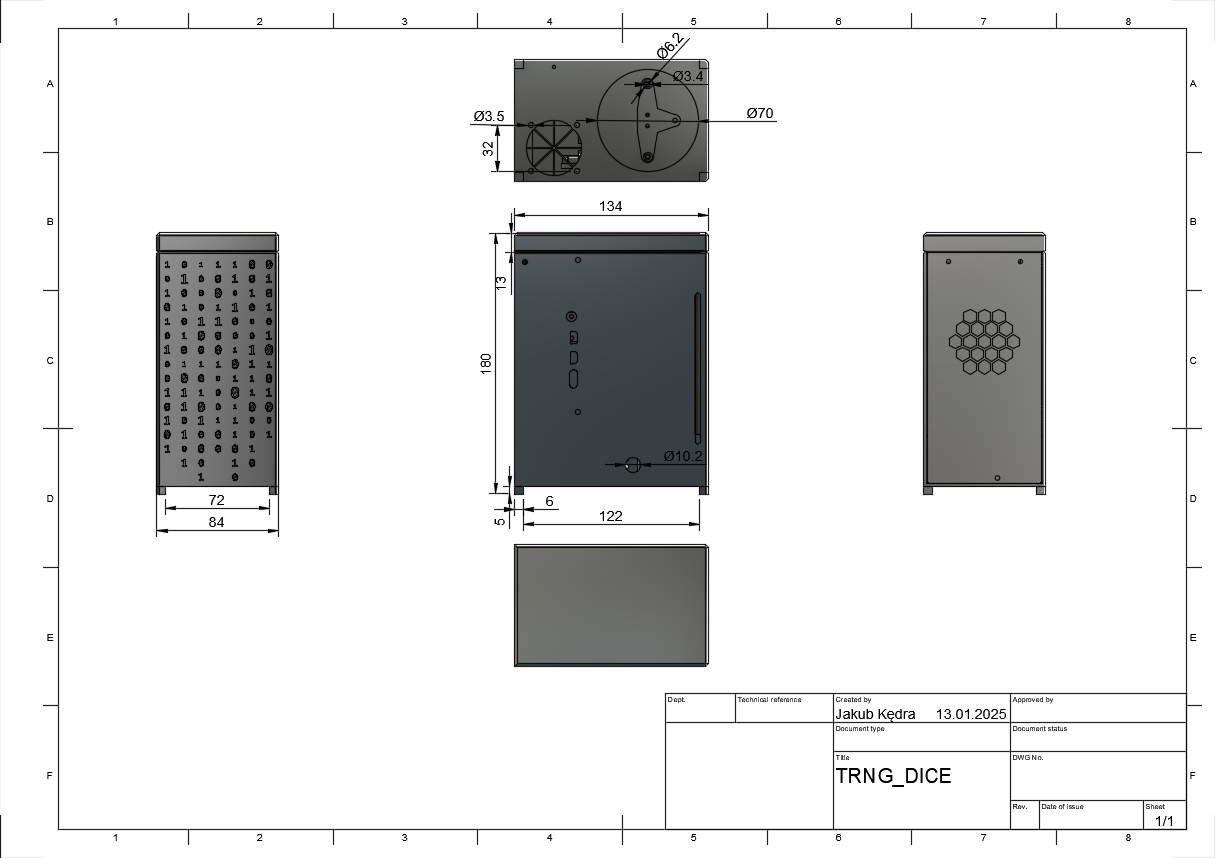
\includegraphics[width=0.95\linewidth]{chapters/03-praca-wlasna/figures/wymiary.png}
    \caption{\label{fig:wymiary}Wymiary zewnętrzne}
\end{figure}

\begin{figure}[H]
    \centering
    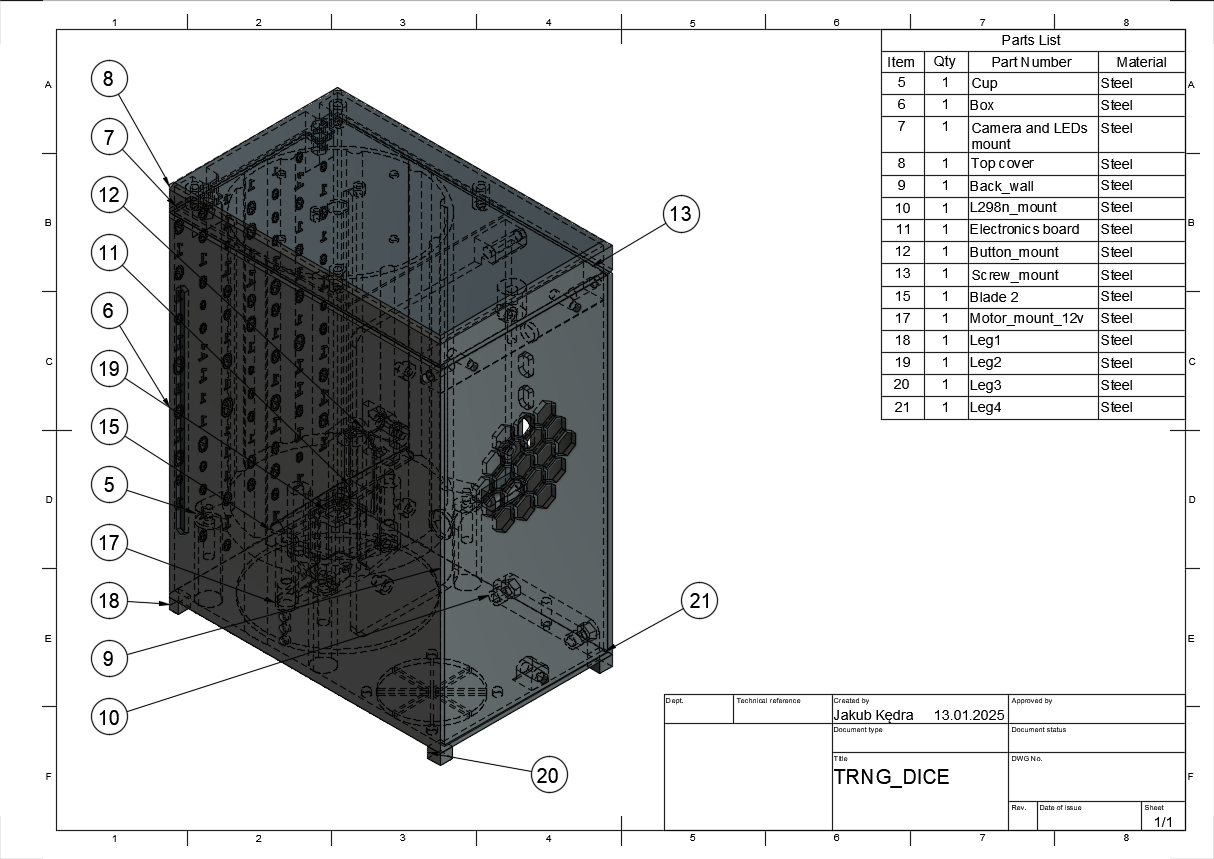
\includegraphics[width=0.95\linewidth]{chapters/03-praca-wlasna/figures/komponenty.png}
    \caption{\label{fig:komponenty}Komponenty robota}
\end{figure}

\begin{figure}[H]
    \centering
    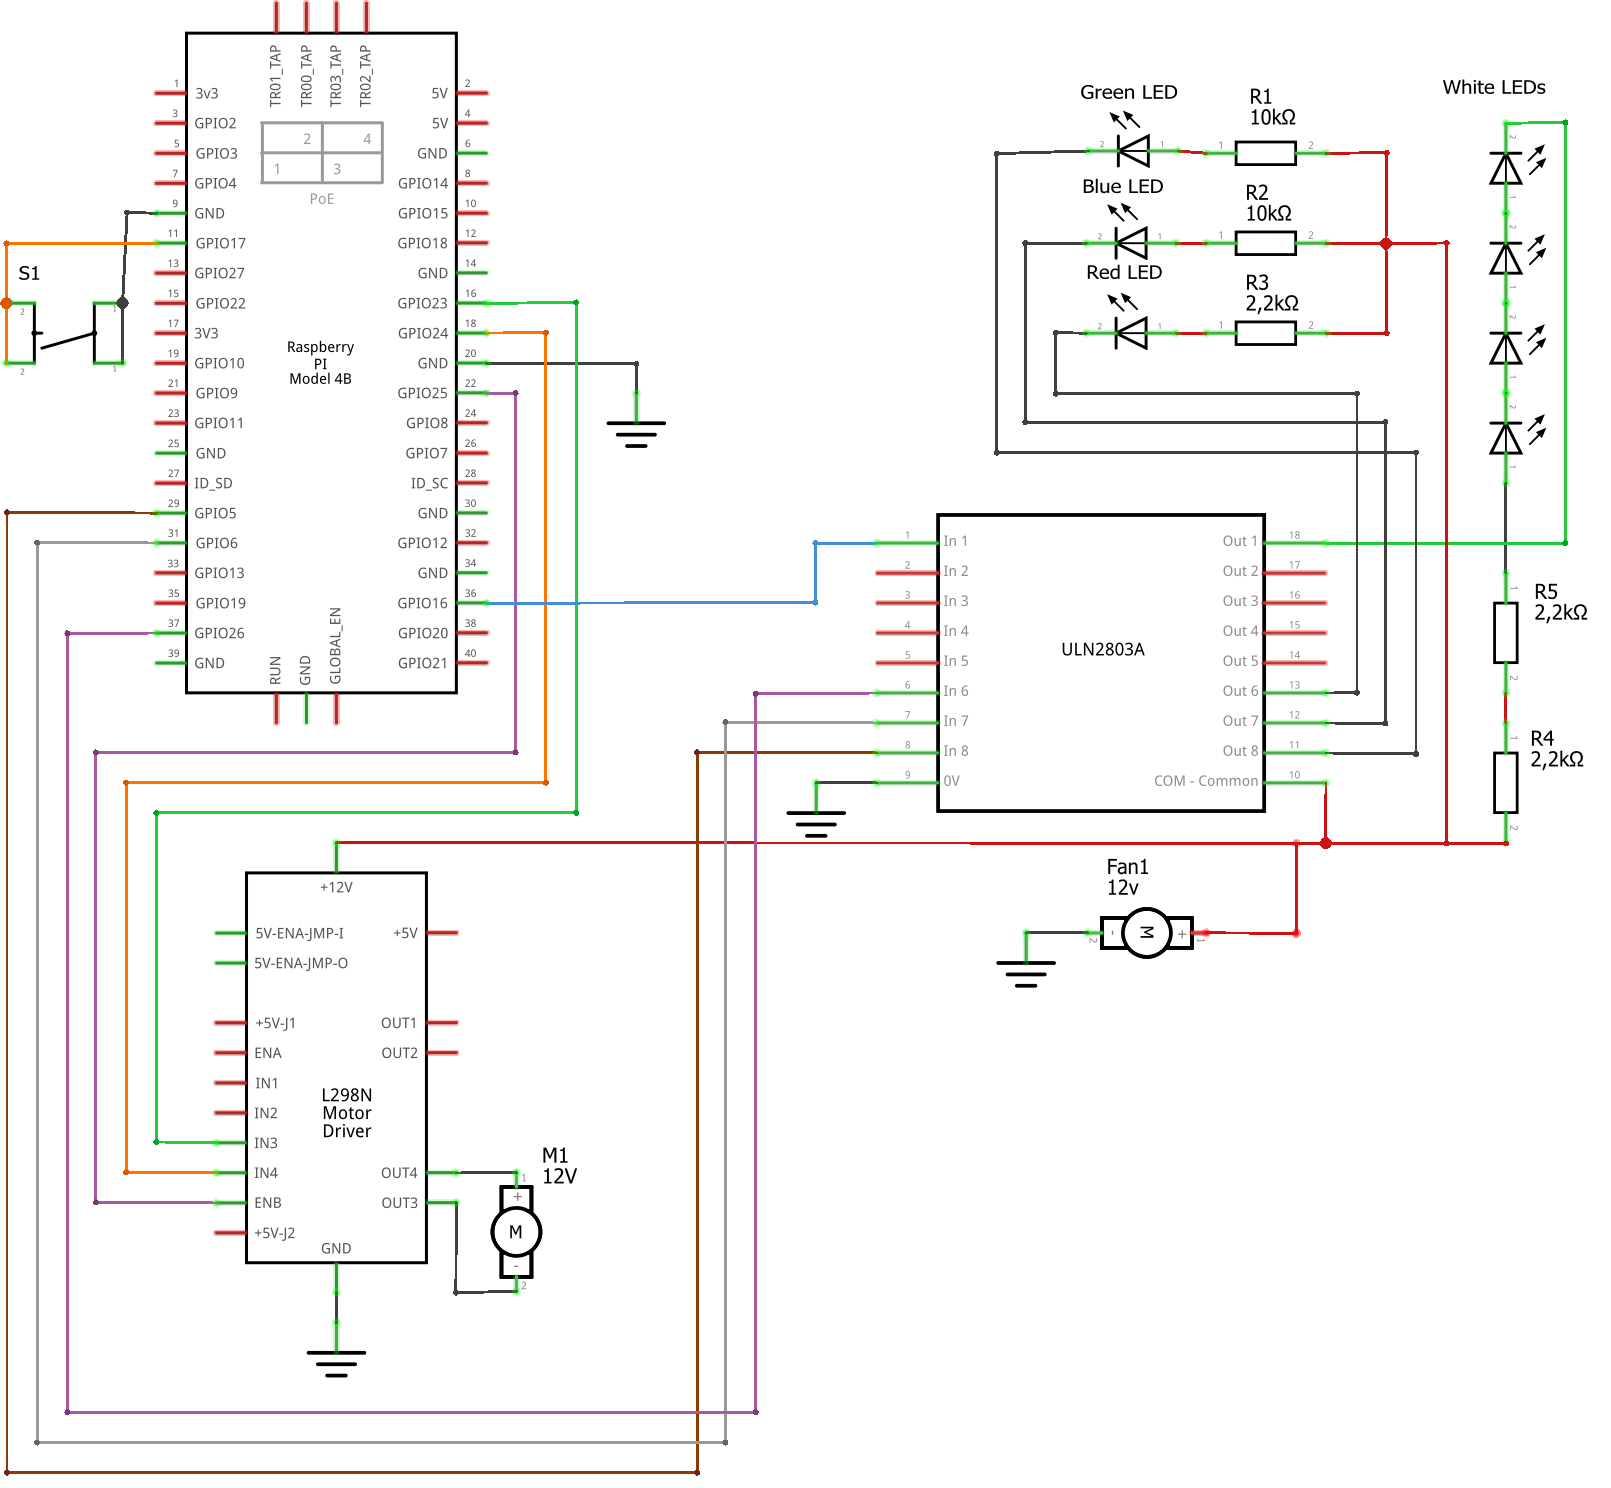
\includegraphics[width=0.95\linewidth]{chapters/03-praca-wlasna/figures/electronics circut_schem.png}
    \caption{\label{fig:electronics}Schemat elektryczny}
\end{figure}

\subsection{Software}
bbbbbbbbbbbbbbbbbbbbb